\appendix
\chapter{}
\section{Data Sources}
The interest rates used for Black-Scholes model and Vanna-Volga model were obtained from \textit{www.tradingeconomics.com} and was listed below.
\begin{figure}[tbph]
	\centering
	\includegraphics[width=0.6\linewidth]{"Testing-data/Interest rate - Trading economics"}
	\caption{Interest rates from tradingeconomics.com}
	\label{fig:interest-rate---trading-economics}
\end{figure}
\newline
The prices of EUR/USD in \textit{www.investing.com} is following:
\begin{figure}[tbph]
	\centering
	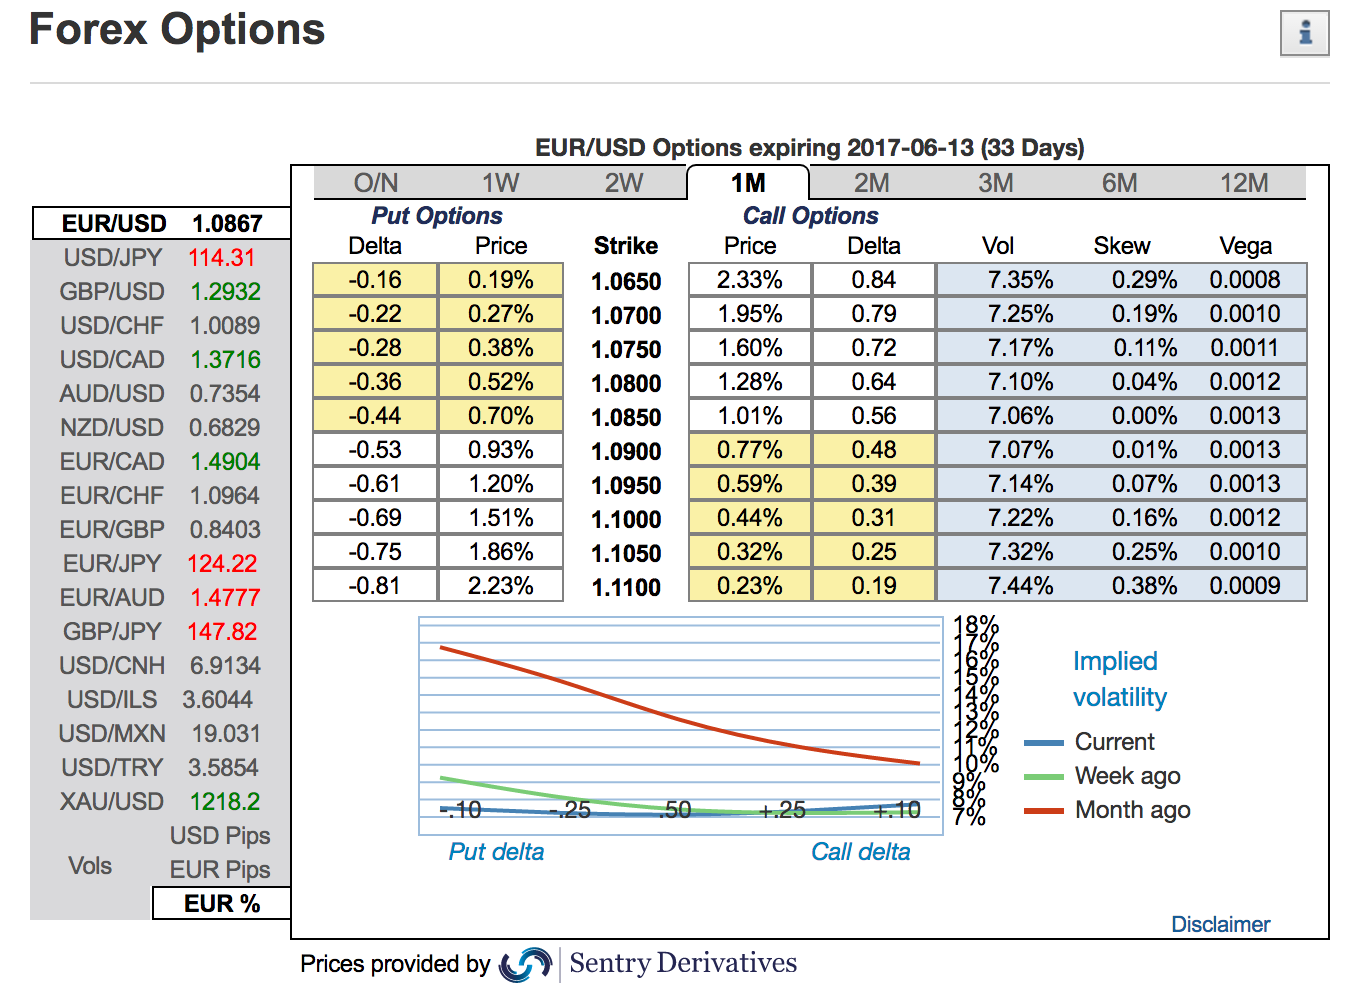
\includegraphics[scale=0.3]{./Testing-data/EURUSD_1M_investing.png} 
	\caption{EUR/USD call prices from investing.com}
	\label{fig:prices-investing.com} % insert suitable label, this is used to refer to a fig from within the text as shown above
\end{figure}
\newline
Since Bloomber has its own pricing model for FX options, the prices of EUR/USD call options with different strikes are obtained in Bloomberg terminal and listed below (using strike 1.065 as example).

\begin{figure}[htb]
	\centering
	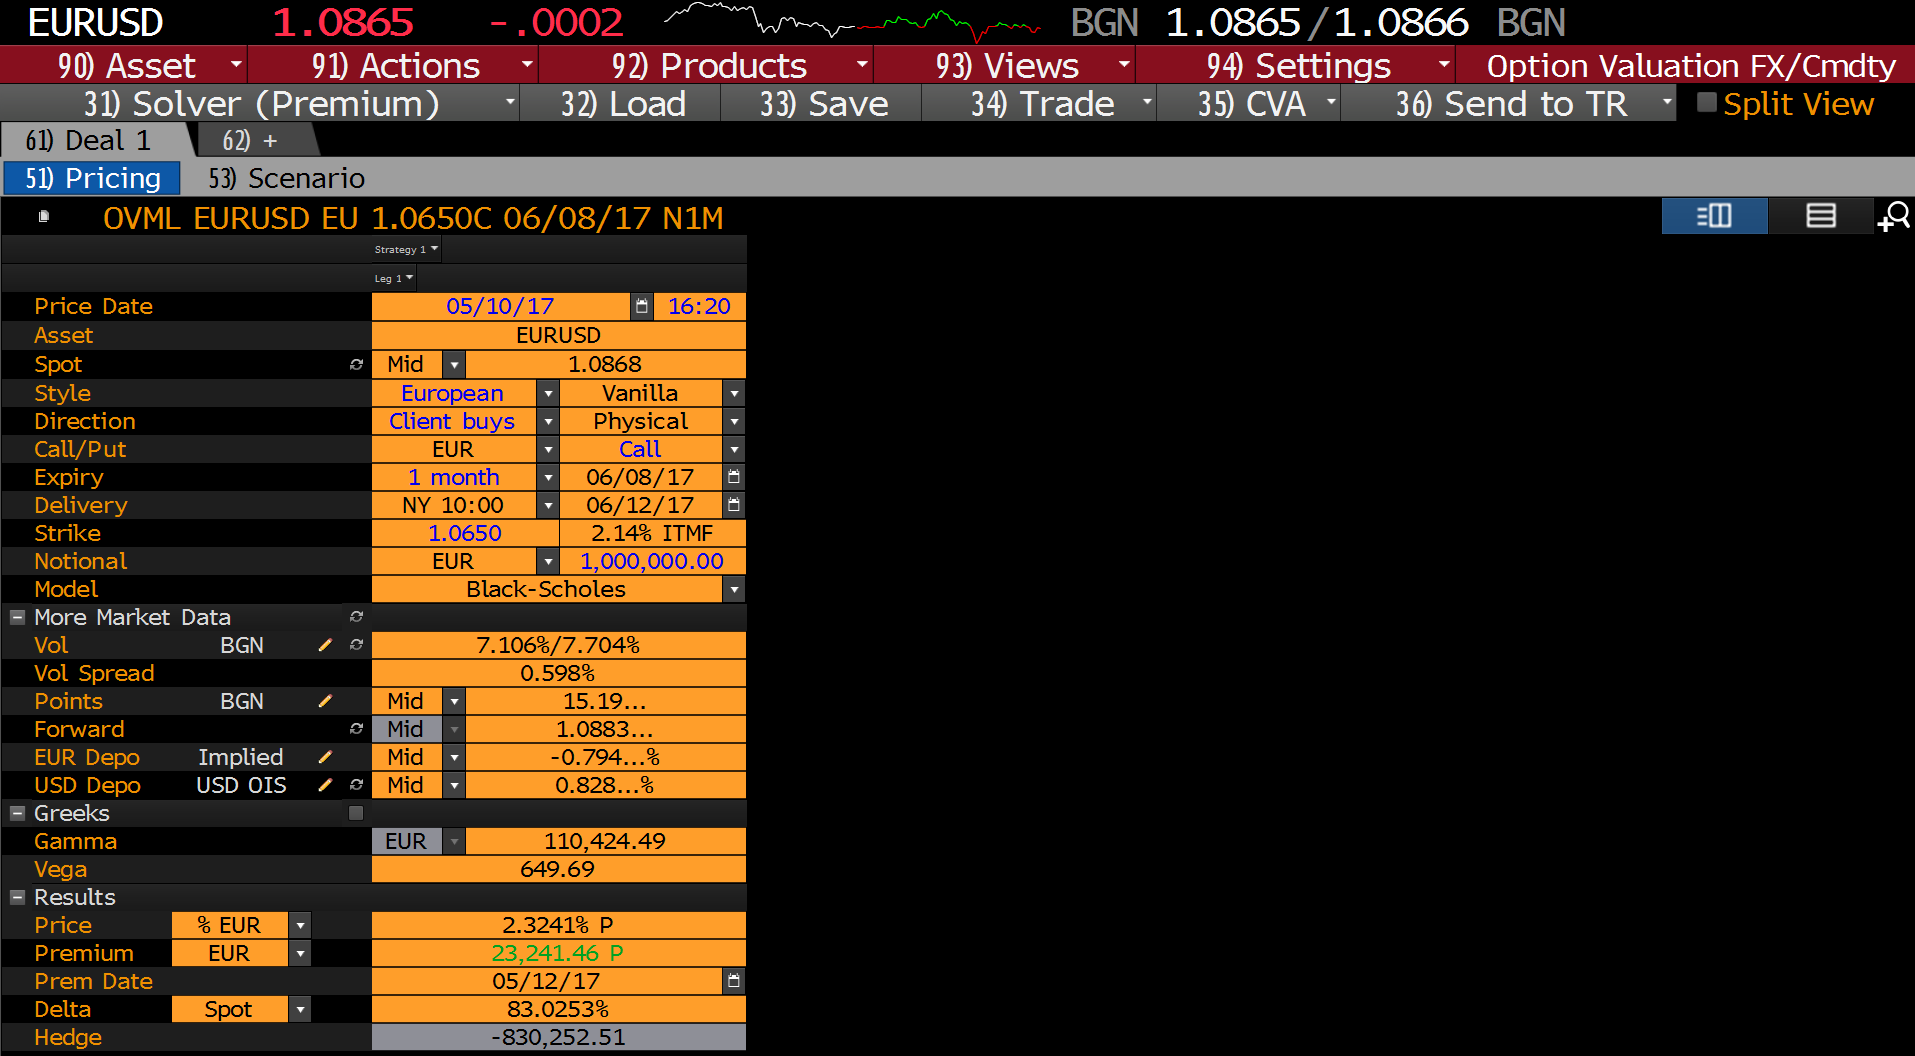
\includegraphics[scale=0.3]{./Testing-data/Price-Bloomberg/EURUSD1065.PNG} 
	\caption{EUR/USD call prices with strike 1.065}
	
	\label{fig:prices-investing.com} % insert suitable label, this is used to refer to a fig from within the text as shown above
\end{figure}

\section{Definitions}
25 and 10 $\Delta$-Risk-reversal (RR) volatility:
\begin{align}
\sigma_{RR25}&=\sigma_{25\Delta C}-\sigma_{25\Delta P}\\
\sigma_{RR10}&=\sigma_{10\Delta C}-\sigma_{10\Delta P}
\end{align}
\newline
25 and 10 $\Delta$-Butterfly (BF) volatility:
\begin{align}
\sigma_{BF25}=\frac{1}{2}\left[\sigma_{25\Delta C}+\sigma_{25\Delta P}\right]-\sigma_{ATM}\\
\sigma_{BF10}=\frac{1}{2}\left[\sigma_{10\Delta C}+\sigma_{10\Delta P}\right]-\sigma_{ATM}
\end{align}
\newline
These yields to the following equations:
\begin{align}
\sigma_{25\Delta C}=\sigma_{ATM}+\sigma_{BF25}+\frac{1}{2}\sigma_{RR25}\\
\sigma_{25\Delta P}=\sigma_{ATM}+\sigma_{BF25}-\frac{1}{2}\sigma_{RR25}\\
\sigma_{10\Delta C}=\sigma_{ATM}+\sigma_{BF10}+\frac{1}{2}\sigma_{RR10}\\
\sigma_{10\Delta P}=\sigma_{ATM}+\sigma_{BF10}-\frac{1}{2}\sigma_{RR10}
\end{align}
\newline
Strike retrived from deltas can be calculated through following equation:
\begin{align}
K=S_0e^{(r_d-r_f)T-\phi \sigma \sqrt{T} N^{-1}(\phi \Delta)+\frac{1}{2}\sigma^2T}
\end{align}
where $\phi=1$ for call, and $\phi=-1$ for put.

\section{Python Code of Vanna-Volga Model}
The codes of Vanna-Volga model had been implemented in jupyter notebook with kernel Python 3.5. Details of the codes could be found in the corresponding jupyter notebook with name as "MTH9845\_final\_project\_codes.ipynb". The jupyter notebook also had been converted to a pdf file with name as "MTH9845\_final\_project\_codes.pdf". Please see the details in the seperate files.
\newline
\newline
The Black-Scholes prices and Vanna-Volga prices calculated by implemented codes had been put in the following figure. The prices from Bloomberg and \textit{inversting.com} were also included.
\begin{figure}[tbph]
	\centering
	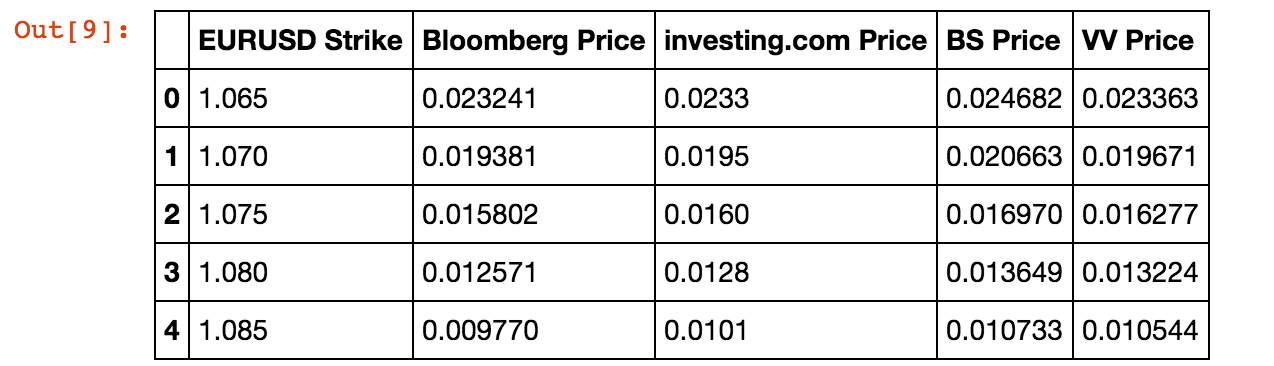
\includegraphics[width=1.0\linewidth]{./Testing-data/prices-python.png}
	\caption{Combined prices of EUR/USD with different strikes}
	\label{fig:prices-python}
\end{figure}
